% 43B(h) Desk -- take-home brief (Tresata). Compile with pdflatex (Overleaf: default settings).
\documentclass[10pt,a4paper]{article}
\usepackage[a4paper,top=12mm,bottom=14mm,left=15mm,right=15mm]{geometry}
\usepackage[T1]{fontenc}
\usepackage[utf8]{inputenc}
\usepackage{lmodern}
\usepackage[scaled=0.92]{helvet}
\renewcommand{\familydefault}{\sfdefault}
\usepackage{microtype}
\usepackage{graphicx}
\usepackage{xcolor}
\usepackage{longtable,booktabs,array,calc}
\usepackage{enumitem}
\usepackage{titlesec}
\usepackage{needspace}
\usepackage{fancyhdr}
\usepackage[hidelinks]{hyperref}
\definecolor{accent}{HTML}{0D6A57}
\definecolor{muted}{HTML}{56635D}
\hypersetup{colorlinks=true,urlcolor=accent,linkcolor=accent}
\setlength{\parindent}{0pt}
\setlength{\parskip}{3.5pt}
\linespread{1.02}
\titleformat*{\section}{\large\bfseries\color{accent}}
\titlespacing*{\section}{0pt}{8pt}{2pt}
\setlist{nosep,leftmargin=13pt,topsep=1pt,itemsep=1.5pt}
\setlength{\LTpre}{3pt}\setlength{\LTpost}{4pt}
\renewcommand{\arraystretch}{1.12}
\providecommand{\tightlist}{\setlength{\itemsep}{1.5pt}\setlength{\parskip}{0pt}}
\pagestyle{fancy}\fancyhf{}\renewcommand{\headrulewidth}{0pt}
\fancyfoot[R]{\scriptsize\color{muted}\thepage}
\newcommand{\sourcesstart}{\begingroup\scriptsize\color{muted}}
\newcommand{\sourcesend}{\endgroup}
\begin{document}
\small
{\LARGE\bfseries 43B(h) Desk --- Take-home brief\par}
\vspace{2pt}
{\footnotesize\color{muted} Shashank Kumar \textperiodcentered{} 2023CS10020 \textperiodcentered{} Computer Science and Engineering, IIT Delhi \textperiodcentered{} 3 Nov 2026\par}
\vspace{4pt}
\textbf{India's 45-day rule turns a late payment to a small supplier into a tax add-back, and deciding which payables it hits means reading documents nobody has digitised. I built a checker where the AI only reads, code applies the law, and a person is asked only when their answer changes the rupee figure.}

Jurisdiction: India (MSMED Act 2006 s.2(b), s.15; Income-tax Act 1961 s.43B(h) to FY 2025-26; Income-tax Act 2025 s.37(2)(g) from tax year 2026-27). All test data is synthetic.

\needspace{7\baselineskip}\section*{1. Area explored, and what surprised me}

Since FY 2023-24 a buyer may deduct a sum owed to a micro or small enterprise only in the year it is paid, if it pays after the MSMED Act limit: 15 days from acceptance, or up to 45 days if agreed in writing. Paying before the return due date does not help.

\begin{itemize}
\tightlist
\item
  \textbf{The rule meant to protect small suppliers also pushed buyers away from them.} Orders reportedly moved to unregistered vendors, and some suppliers gave up their Udyam registration. A Rajya Sabha question raised this in July 2026; the reply gave no data.
\item
  \textbf{Paying late does not, by itself, cost tax.} Only an amount unpaid on 31 March and then paid after its due date, or not at all, is added back. The work concentrates on year-end payables and on one date ERPs rarely hold: the day of acceptance.
\item
  \textbf{The ground is moving.} From tax year 2026-27 the rule is s.37(2)(g) and Form 3CD becomes Form 26. Parts of the MSMED (Amendment) Act 2026 took effect on 15 Oct 2026; reports say the 15/45-day rule is unchanged. Limits rose on 1 Apr 2025; many guides still quote the old ones.
\end{itemize}

\needspace{7\baselineskip}\section*{2. The problem}

\textbf{Each year a buyer's finance team and its tax auditor (a CA) must decide, invoice by invoice, which payables to micro and small suppliers are disallowed. They do it by hand.}

\begin{itemize}
\tightlist
\item
  \textbf{Who and how often:} a mid-size buyer that needs a tax audit, and the CA who signs it. Once a year; the same data feeds half-yearly MSME-1 returns and the annual-accounts disclosure.
\item
  \textbf{Task:} for each payable to a micro or small supplier unpaid on 31 March, decide whether, and how much, is disallowed; report it in Form 3CD clause 22 (Form 26 from 2026-27).
\item
  \textbf{Why it is hard:} three facts live in documents, not the ERP. Is the supplier micro or small, and not a trader, for that year (Udyam certificate row and NIC code)? What payment term was agreed in writing (a PO clause, or only a line on the supplier's invoice)? When were the goods accepted (delivery, unless a written objection within 15 days moved it)?
\item
  \textbf{Cost today:} emailing vendors for certificates, reading POs, a spreadsheet. My unvalidated estimate: 100+ person-hours for 300 small-supplier vendors and 1,000 open invoices. Errors cut both ways: over-stating pays tax a year early; under-stating brings a demand with interest, under the CA's signature. At the 25.17\% company rate, each Rs~1 crore misclassified moves about Rs~25 lakh of tax between years.
\end{itemize}

\textbf{Why it matters, and why now.} Small enterprises have 2,56,892 delayed-payment cases worth Rs~55,244 crore on the government's Samadhaan portal, Rs~20,979 crore still pending (14 Aug 2026). Late payment also carries non-deductible MSMED s.16 interest at three times the bank rate, compounded monthly: 17.25\% a year since the 7 Oct 2026 rate hike. Tax year 2026-27 brings a new Act and a new audit form, so every firm's working papers change now.

\textbf{Out of scope:} computing s.16 interest; the GST part of invoices; verifying certificates on the Udyam portal; the supplier's side; MSME-1 filing; and any decision the law leaves to a qualified person, which the tool asks rather than answers.

\needspace{7\baselineskip}\section*{3. Solution design}

\textbf{The LLM turns documents into quoted facts. Code checks every quote, applies a dated rule pack and recomputes the figure under every reading that survives. The CA sees only invoices whose figure depends on a doubt.}

\begin{itemize}
\tightlist
\item
  \textbf{In:} Udyam certificate, PO or contract, supplier invoice, QC and email notes; GRN, invoice and payment dates and amounts from the ERP.
\item
  \textbf{The AI:} extracts five facts per vendor (type for the year, activity, registration date, payment term, written objections), each with a verbatim quote and any other defensible reading. It never computes a date or decides whether the law applies.
\item
  \textbf{Out:} per invoice, the amount disallowed, the rule ids and citations behind it, and the quotes; totals for Form 3CD clause 22 or Form 26.
\item
  \textbf{A person:} answers review questions, decides each judgment call once for the firm, and signs the rule pack and the working paper.
\end{itemize}

\begin{center}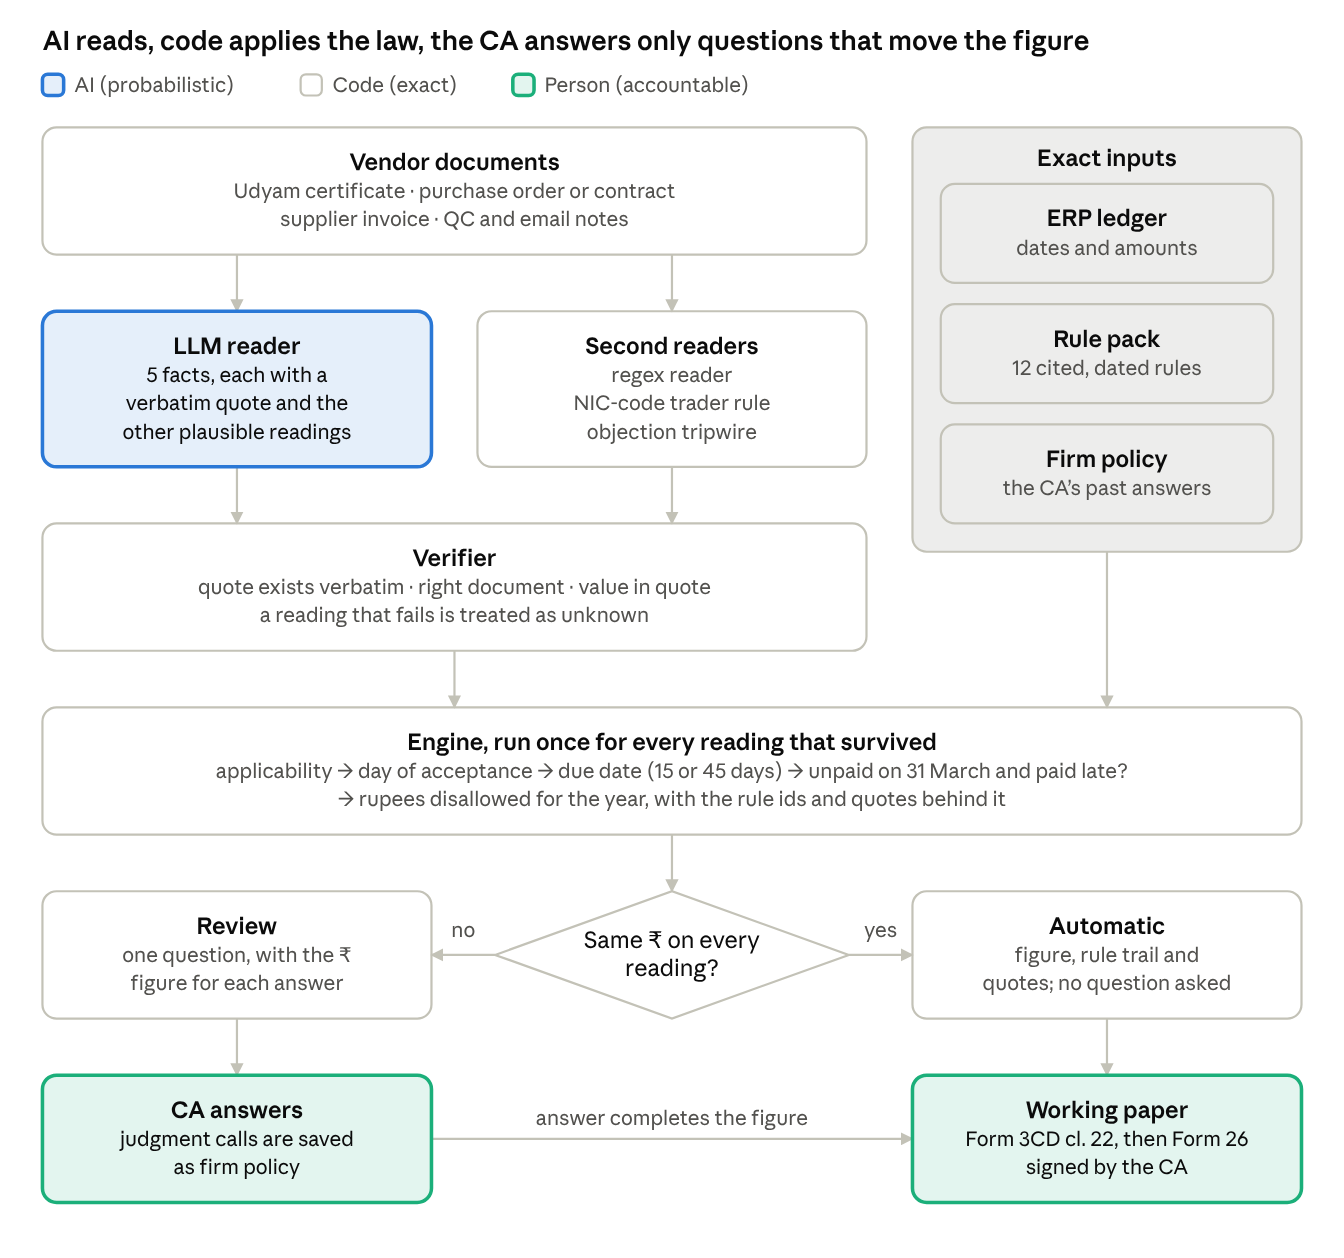
\includegraphics[width=0.66\linewidth]{architecture.png}\end{center}\vspace{-4pt}

The only probabilistic box is the LLM reader; every arrow into the engine carries an exact input or a verified quote.

\needspace{7\baselineskip}\section*{4. Exact versus probabilistic, and how uncertainty is handled}

\textbf{Only reading the documents is probabilistic. Everything that produces a rupee figure is code, and every reading it uses carries a verbatim quote.}

\begin{longtable}[]{@{}
  >{\raggedright\arraybackslash}p{(\columnwidth - 6\tabcolsep) * \real{0.2500}}
  >{\raggedright\arraybackslash}p{(\columnwidth - 6\tabcolsep) * \real{0.2500}}
  >{\raggedright\arraybackslash}p{(\columnwidth - 6\tabcolsep) * \real{0.2500}}
  >{\raggedright\arraybackslash}p{(\columnwidth - 6\tabcolsep) * \real{0.2500}}@{}}
\toprule\noalign{}
\begin{minipage}[b]{\linewidth}\raggedright
Part
\end{minipage} & \begin{minipage}[b]{\linewidth}\raggedright
Exact?
\end{minipage} & \begin{minipage}[b]{\linewidth}\raggedright
Lives in
\end{minipage} & \begin{minipage}[b]{\linewidth}\raggedright
When it goes stale
\end{minipage} \\
\midrule\noalign{}
\endhead
\bottomrule\noalign{}
\endlastfoot
The law: 15/45 days, acceptance, 31 March test, which Act and form & Exact & 12 cited rules in code, each with an FY window & At its review date; the engine refuses to run after it \\
Judgment calls (invoice-only terms, capital purchases) & Exact once decided & Policy file signed by the CA & When the CA changes it \\
Dates and amounts & Exact & ERP ledger & n/a \\
What a document says & Probabilistic & LLM reading, with quotes & Per document \\
Whether a doubt matters & Exact & Rupee sensitivity check & n/a \\
\end{longtable}

\textbf{Uncertainty is measured in rupees, not model confidence.} The engine runs on every reading that survives the guards: the LLM's, its alternates, the regex reader's when it differs, and the full range when a guard fails. Same disallowance on every run: settled automatically. Different: one question, with the rupee figure for each answer. Confidence scores are poorly calibrated, and a confident reading can still be a legal judgment.

\begin{itemize}
\tightlist
\item
  \textbf{Unknown fact, no question.} A canteen contract pays ``15 days from certification of the monthly bill''; the date is nowhere. The bill was paid 55 days after service, past the 45-day cap on any reading, so Rs~1,10,000 is settled without asking.
\item
  \textbf{Clear text, still a question.} A term printed only on the supplier's invoice: is it an agreement ``in writing''? The CA decides once (Rs~0 or Rs~2,95,000 here) and the answer becomes firm policy.
\end{itemize}

Disallowance can only fall as the due date moves later, so a doubt about a date needs only its earliest and latest readings.

\textbf{Mistakes are caught before the engine.} A quote must exist verbatim in the named document. It must come from the right kind of document: enterprise type only from the Udyam certificate, which also defeats instructions planted in a PO. It must contain the value it supports: the date, the days (in digits, words or Hindi), the right FY row. A payment term must come from a sentence about payment. A fact that fails becomes unknown; it is never used silently.

\textbf{Why AI at all.} A careful regex reader got the payment term right for 12 of 18 vendors. It missed terms in words or Hindi, an objection dated ``Thu, 12 Mar 2026'', a trader whose certificate says ``Services'', and a delivery period inside the payment sentence. Real POs vary far more. Today a person reads them; the AI replaces that reading and nothing else.

\needspace{7\baselineskip}\section*{5. What I considered and rejected}

\begin{longtable}[]{@{}
  >{\raggedright\arraybackslash}p{(\columnwidth - 2\tabcolsep) * \real{0.5000}}
  >{\raggedright\arraybackslash}p{(\columnwidth - 2\tabcolsep) * \real{0.5000}}@{}}
\toprule\noalign{}
\begin{minipage}[b]{\linewidth}\raggedright
Option
\end{minipage} & \begin{minipage}[b]{\linewidth}\raggedright
Why not
\end{minipage} \\
\midrule\noalign{}
\endhead
\bottomrule\noalign{}
\endlastfoot
One LLM call: ``how much is disallowed?'' & Law and date arithmetic inside the model; no trail an auditor can check; answers can drift between runs. \\
Retrieval over the Act & The law here is about twelve sentences. As code it is cited and tested; retrieval adds a failure mode, not knowledge. Retrieval stays useful for vendor documents. \\
Several agents (reader, ``lawyer'', calculator) & More places to be wrong. The ``lawyer'' is better as rules a CA can read in ten minutes. \\
Escalate on low model confidence & Poorly calibrated, and blind to whether the fact matters. \\
Rules and regex only & 6 of 19 invoices got a wrong figure with no warning. Kept as a second reader. \\
Fine-tuning a model & No labelled data, and the law changes yearly. Judgments go to a policy file. \\
Vendor self-declarations & Useful, but they give no payment terms or acceptance dates, and still need checking. \\
\end{longtable}

\needspace{7\baselineskip}\section*{6. Risks}

\textbf{The weakest point is a misreading two readers share.} If the LLM reads ``material to be delivered within 30 days of this order; payment as per our usual practice'' as a 30-day payment term, the quote is real, mentions payment and contains 30, and the regex reader agrees. Nothing flags it. It is the one silent error left in fault injection. Next to try: a second model family, and a check on which noun the number belongs to.

\begin{longtable}[]{@{}
  >{\raggedright\arraybackslash}p{(\columnwidth - 4\tabcolsep) * \real{0.3333}}
  >{\raggedright\arraybackslash}p{(\columnwidth - 4\tabcolsep) * \real{0.3333}}
  >{\raggedright\arraybackslash}p{(\columnwidth - 4\tabcolsep) * \real{0.3333}}@{}}
\toprule\noalign{}
\begin{minipage}[b]{\linewidth}\raggedright
Risk
\end{minipage} & \begin{minipage}[b]{\linewidth}\raggedright
How the design handles it
\end{minipage} & \begin{minipage}[b]{\linewidth}\raggedright
What is left
\end{minipage} \\
\midrule\noalign{}
\endhead
\bottomrule\noalign{}
\endlastfoot
Wrong answers & Quote guards, rupee sensitivity, a second reader, a NIC-code rule and an objection tripwire. In 154 injected-error runs, silent wrong figures fell from 60 to 1. & Shared misreadings; real documents are messier than mine. \\
Outdated rules & Dated, cited rule pack; one test per rule; the engine stops after the review date; a watch-list names pending changes. & A person must re-verify on time. \\
Confidential data & Send only the four document types, bank and PAN numbers masked. In production, a model in the firm's own tenancy or self-hosted; free hosted models only for synthetic data. & Documents still leave the ERP. \\
Liability, tax advice & The tool prepares working papers. The CA who signs the audit report stays accountable, signs the rule pack and policy, and answers every judgment call. Each figure shows its rule and quote. & Rubber-stamping; the desk shows what was automatic and why. \\
Fake or stale certificate & Production should verify the Udyam number on the government portal. & Not built. \\
\end{longtable}

\needspace{7\baselineskip}\section*{7. Prototype: what I built and where it fails}

\textbf{A dependency-free Python prototype and a clickable review desk (\texttt{desk/review\_desk.html} in the repo), tested on 18 synthetic vendors (19 invoices) that I wrote and labelled by hand.} The cases cover the 45-day cap, no written term, a trader, a supplier that became Medium, objections inside and outside 15 days, terms in words and in Hindi, an invoice-only term, late registration, a capital purchase, part-payments and a prompt injection.

\begin{longtable}[]{@{}
  >{\raggedright\arraybackslash}p{(\columnwidth - 2\tabcolsep) * \real{0.5000}}
  >{\raggedright\arraybackslash}p{(\columnwidth - 2\tabcolsep) * \real{0.5000}}@{}}
\toprule\noalign{}
\begin{minipage}[b]{\linewidth}\raggedright
Test
\end{minipage} & \begin{minipage}[b]{\linewidth}\raggedright
Result
\end{minipage} \\
\midrule\noalign{}
\endhead
\bottomrule\noalign{}
\endlastfoot
Engine against my hand-computed answers & 19 of 19 \\
Regex reader alone & 6 of 19 get a wrong figure with no warning \\
Correct reading with guards and cross-checks & 16 automatic and right; the invoice-only term correctly asked; 2 extra reviews from the second reader \\
\end{longtable}

\textbf{Fault injection} tests the guards rather than one model: one LLM-style error per run (an invented quote, a wrong value with a real quote, the wrong clause, a missed objection) on otherwise-correct facts. 154 runs.

\begin{longtable}[]{@{}llll@{}}
\toprule\noalign{}
Setup & Right, automatic & Sent to review & Wrong, no flag \\
\midrule\noalign{}
\endhead
\bottomrule\noalign{}
\endlastfoot
Trust the reader & 94 & 0 & 60 \\
Guards + rupee sensitivity & 83 & 67 & 4 \\
+ second reader, NIC rule, tripwire & 80 & 73 & 1 \\
\end{longtable}

The evaluation changed the design. The first run left 4 silent errors. Two came from a trader whose certificate says ``Services''; I moved that signal from the prompt into code (every NIC code in divisions 45 to 47 means a trader). One was a missed objection, which no quote check can catch; I added a tripwire on objection words in the notes.

\textbf{Where it fails.} (1) The shared misreading in section 6. (2) I wrote the cases, so they test the rules, not scans, tables or multi-PO contracts. (3) Fault injection measures the guards against errors I chose, not how often a real model makes them. (4) The live run on a free OpenRouter model (\texttt{eval/run\_eval.py\ -\/-llm}) has not been run yet; the harness, prompt and response cache are ready. (5) The second reader costs 2 reviews in 19 even with a perfect reading.

\needspace{7\baselineskip}\section*{8. Other jurisdictions, and what I would do before spending more time}

\textbf{Another country changes the rule pack and the supplier registry; the reader, guards and sensitivity check carry over.} India is unusual in tying late payment to tax deductibility. Elsewhere the same pipeline would produce a late-payment interest claim or a payment-practices report instead of a tax add-back.

\begin{enumerate}
\def\labelenumi{\arabic{enumi}.}
\tightlist
\item
  \textbf{Practitioners first.} An hour each with a manufacturer's accounts team and a tax auditor, plus a dozen redacted POs, certificates and QC emails, to test my assumptions and the real time cost.
\item
  \textbf{Two model families on real documents,} counting the mistakes they share. That number decides whether the weakest point is acceptable.
\item
  \textbf{Udyam portal checks and ERP feeds} for certificates, the vendor master and GRN dates. Linking one supplier across the vendor master, its Udyam certificate, GSTIN and PAN is an entity-resolution problem that must be solved before any rule runs.
\item
  \textbf{Check the amended MSMED text in the gazette;} map outputs to Form 26; add s.16 interest.
\end{enumerate}

\vspace{6pt}
\sourcesstart\textbf{Sources.} Law and forms: \href{https://taxguru.in/income-tax/finance-ministry-clarifies-section-43bh-45-day-msme-payment-rule.html}{Rajya Sabha reply on s.43B(h) and s.37(2)(g), 21 Jul 2026 (TaxGuru)} \textperiodcentered{} \href{https://taxclue.in/blog/section-37-income-tax-act-2025-actual-payment-basis}{s.37 of the Income-tax Act 2025 (Taxclue)} \textperiodcentered{} \href{https://www.taxscan.in/top-stories/msme-payment-rule-us-43bh-of-income-tax-act-due-dates-tax-impact-and-form-3cd-reporting-1449695}{MSME rule and tax impact (Taxscan, 4 Aug 2026)} \textperiodcentered{} \href{https://www.india-briefing.com/news/msme-tax-audit-form-3cd-clauses-22-26-fy-2025-26-47290.html/}{Form 3CD clauses 22 and 26 (India Briefing)} \textperiodcentered{} \href{https://cleartax.in/s/form-26-tax-audit}{Form 26 under rule 47 (ClearTax)} \textperiodcentered{} \href{https://www.snrlaw.in/payments-to-micro-and-small-enterprises-mses-implications-under-section-43bh-of-income-tax-act-1961/}{Acceptance, traders, interest (S\&R Associates)} \textperiodcentered{} \href{https://newsonair.gov.in/govt-notifies-revised-criteria-for-classifying-msmes}{Revised MSME limits from 1 Apr 2025 (News On AIR)} \textperiodcentered{} \href{https://www.corpseed.com/law-update/msmed-amendment-act-2026-treds-registration-payment-penalties}{MSMED (Amendment) Act 2026, assent 13 Aug 2026 (Corpseed)} \textperiodcentered{} \href{https://taxguru.in/corporate-law/msme-amendment-act-2026-sections-effective-15-october-15-december.html}{Commencement from 15 Oct and 15 Dec 2026 (TaxGuru)} \textperiodcentered{} \href{https://ibclaw.in/msme-development-amendment-act-2026-commencement-notification-no-so-5575e-dated-12-10-2026/}{Notification S.O. 5575(E), 12 Oct 2026 (IBClaw)} \textperiodcentered{} \href{https://busy.in/business-updates/msme-amendment-bill-2026-what-businesses-should-know/}{Trader clarification of 28 Jun 2024 (Busy)} \textperiodcentered{} \href{https://taxclue.in/news/rbi-raises-repo-rate-by-25-bps-to-5-50-changes-stance-to-calibrated-tightening-sdf-5-25}{RBI rates from 7 Oct 2026 (Taxclue)}.\par
Impact: \href{https://moneylife.in/article/45days-payment-security-clause-creating-hurdles-for-msmes-as-companies-place-orders-with-unregistered-players-sc-allows-vyapar-mandal-to-move-hc-reports/74097.html}{Buyers shifting to unregistered vendors (Moneylife, 6 May 2024)} \textperiodcentered{} \href{https://www.taxscan.in/other-taxations/rajya-sabha-notes-impact-of-section-43bh-of-finance-act-2023-on-msme-payments-and-buyer-evasion-read-order-1449331}{Rajya Sabha on buyer evasion (Taxscan, 26 Jul 2026)} \textperiodcentered{} \href{https://intelligence.crisil.com/en/homepage/newsroom/press-releases/2026/08/executed-well-msme-bill-can-be-an-ibc-moment-for-delayed-payments.html}{Samadhaan figures as of 14 Aug 2026 (Crisil Intelligence)}. Not legal or tax advice.\par\sourcesend

\clearpage
\section*{Appendix: what I added beyond the AI}

{\footnotesize\color{muted} Logs attached: my Google Gemini conversation ``AI Finance Assignment Ideas'' (87 pages: choosing the problem, learning the law, the architecture, a review of each module).\par}

\textbf{Where AI helped.} (1) Finding the problem: Gemini offered audit vouching, transfer-pricing comparables, beneficial-owner unrolling, s.194R TDS, GSTR-2B credit matching and s.43B(h). I picked 43B(h) because the answer is one exact rupee figure, the hard inputs are documents, and the law is short enough to write as code. (2) Learning the domain fast: the rule, the CA's year-end routine, where it is reported, how messy real wording gets. (3) A sounding board for the architecture and a reviewer for each module. Three key prompts (verbatim, trimmed):
\begin{itemize}
\item ``Write the full decision tree for 43B(h) as plain rules, step by step: when a supplier counts as micro or small, how traders and late Udyam registration are treated, how the day of acceptance is decided, how written objections within 15 days\,\ldots''
\item ``Model confidence scores aren't reliable. Instead of trusting them, can I run the calculation on every plausible reading of the facts (the LLM's answer, its alternatives, and a regex reader's answer) and only send a case to a human when the\,\ldots''
\item ``Since a CA legally signs the audit report, where exactly should the human be in this system? Some points are unsettled law, like whether a payment term printed only on the supplier's invoice counts as a written agreement. How do\,\ldots''
\end{itemize}

\textbf{What I rejected or corrected, and how I knew.}
{\footnotesize
\begin{longtable}[]{@{}
  >{\raggedright\arraybackslash}p{(\columnwidth - 2\tabcolsep) * \real{0.31}}
  >{\raggedright\arraybackslash}p{(\columnwidth - 2\tabcolsep) * \real{0.69}}@{}}
\toprule\noalign{}
What the AI said & What I did instead, and how I knew \\
\midrule\noalign{}
\endhead
\bottomrule\noalign{}
\endlastfoot
Late payment is ``permanently disallowed'' with ``severe tax penalties'' & Wrong. The section allows the deduction in the year the sum is actually paid, so it is a timing difference. The brief prices it as tax paid a year early, or a demand with interest if under-stated. \\
Year-end test: ``unpaid on 31 March and due date before 31 March $\Rightarrow$ disallow'' & Misses a sum due in April and paid after its due date, which is also disallowed. Case C02 (60-day term capped to 45, due 6 Apr, paid 15 Apr) would show Rs~0 instead of Rs~9,80,000. \\
Fuzzy quote matching, pass at 92--95\% similarity & A quote with one digit changed (``Net 80'' for C02's ``Net 60'') scores 97.6 and passes, and that is the error the guard exists for. I use an exact match after normalising whitespace and Unicode; OCR noise goes to review. \\
Kill switch on today's date, rule void after 1 Apr 2026 & It would block the FY 2025-26 audit, which happens April to September 2026. The law follows the year of the transaction: each rule has an FY window; only the pack's review date depends on today. \\
Its fault-injection harness & It compared each mutated figure with the ground truth, which a real system never sees, never incremented its silent-failure counter, printed ``100\%'', and modelled prompt injection as a zeroed invoice amount, though amounts come from the ERP. Mine injects errors into the reader's output only and scores against hand labels the pipeline cannot see. \\
Sensitivity by shifting payment dates $\pm$5 days and forcing the 15-day default & Payment dates are exact ledger data; perturbing them invents doubt and floods the review queue. I vary only facts read from documents. \\
``Very large'' generated test set: 50 cases with model-written answers & Answers written by the model test the engine against the model. I kept 18 cases and labelled them by hand. \\
A runtime error ``fixed'' with \texttt{.get()} defaults; code called ``an absolute masterpiece'' while it had syntax errors & Here a silently defaulted fact is a wrong rupee figure, so a missing fact becomes unknown and goes to review. I treated praise as no signal and trusted the tests. \\
\end{longtable}}

\textbf{What came from me.}
\begin{itemize}
\item \textbf{Doubt measured in rupees, not confidence} (the second prompt; Gemini only named it). Then: disallowance can only fall as the due date moves later, so a term tied to an undated event needs just its earliest and latest dates. That is how C17 settles Rs~1,10,000 without a question.
\item \textbf{Judgment calls kept out of the model:} the invoice-only term is decided once by the CA as firm policy, never by the model and never per invoice.
\item \textbf{The attack cases:} a delivery period next to the word payment, a trader declaring ``Services'', a Hindi clause in Devanagari (as a real PO would carry it, not Gemini's romanised line), an injected instruction in a PO, a term tied to an undated event. I defend the injection by where a fact may come from (enterprise type only from the Udyam certificate), not by prompt wording.
\item \textbf{Letting the evaluation change the design:} Gemini mentioned the NIC trader codes; after fault injection I moved that check from the prompt into code, added the objection tripwire, and accepted 2 extra reviews in 19 as the price of a second reader.
\end{itemize}

\textbf{One thing I'd defend without AI: the calculation by hand.} C07: goods delivered 1 Feb 2026. The written complaint is dated 21 Feb, day 20, outside the 15-day window, so acceptance stays 1 Feb. The PO says ``45 days from date of receipt'': due 18 Mar. Unpaid on 31 Mar, paid 10 Apr: all Rs~3,60,000 is disallowed for FY 2025-26 and deducted in 2026-27. Had the complaint come by 16 Feb and been closed on 1 Mar, acceptance moves to 1 Mar, the due date to 15 Apr, the payment is on time, and the figure is Rs~0. One date in an email moves Rs~3.6 lakh, which is why that date needs a verified quote and a tripwire, not a confidence score.

\end{document}
